
% ----- preamble -----
% {{{
\documentclass[journal=mamobx, layout=twocolumn]{achemso}

\usepackage{lipsum} % for generating dummy text
\usepackage[dvipsnames]{xcolor} % for colors
\usepackage{graphicx} % for figures
\usepackage{amsmath, amssymb} % for math
\usepackage{bm} % for bold math fonts
\usepackage{xr} % crossreferencing main manuscript to and from supporting info
\externaldocument[SI:]{suppinfo}
% }}}

% --- Title, Author Info, Abstract Text ---
% {{{
\title{How to Write a Research Paper}
\author{Douglas R. Tree}
\affiliation{Chemical Engineering Department, Brigham Young University, Provo, Utah}
\date{\today}
\email{tree.doug@byu.edu}

\newcommand*{\abstracttext}{
% Put abstract text here
\lipsum[1]
}

% for single column abstract
\let\oldmaketitle\maketitle
\let\maketitle\relax
% }}}

% ----- document text -----
\begin{document}

% Format the abstract (make one column, much better looking...)
% {{{
\twocolumn[
\begin{@twocolumnfalse}
  \oldmaketitle
  \begin{abstract}
    \abstracttext
  \end{abstract}
\end{@twocolumnfalse}
]
% }}}

\section{Introduction}
% {{{

Congratulations, you are preparing to write a paper.
Writing a paper is one of the most important parts of doing research.
It is how data gets transmitted to the scientific community and how you get credit for doing the work.

Good researchers start writing the paper while they are planning and executing their research.

Steps to writing a paper:
\begin{enumerate}
  \item Write an introduction
  \item Outline/layout the figures
  \item 
\end{enumerate}


% }}}

\section{Methods}
% {{{

Methods sections often have equations.
Here 
\begin{equation} \label{eq:pythagorus}
a^{2} + b^{2} = c^{2}
\end{equation}
is an example.
Equations should be parts of complete sentences.

You can refer to Eq.~\ref{eq:pythagorus} this way.

% }}}

\section{Results and Discussion}
% {{{

This is an example figure.
You can reference Figure~\ref{fig-placeholder} this way.

\begin{figure}[tbp]
  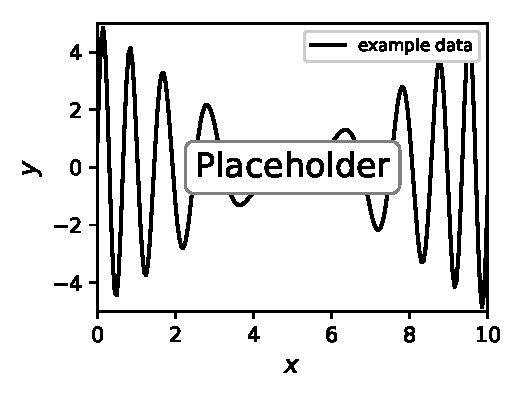
\includegraphics[width=3.25in]{fig-placeholder}
  \caption{Placeholder figure.}
  \label{fig-placeholder}
\end{figure}

Practice citation~\cite{Tree2018}

% }}}

\section{Conclusion}
% {{{
% }}}

\begin{acknowledgement}
% {{{
% Acknowledgements of funding go here
We would like to acknowledge financial support from Brigham Young University and computational resources from the BYU Office of Research Computing.
% }}}
\end{acknowledgement}

\bibliography{refs}

\end{document}
